\section{解決策}

\begin{frame}
  \center
  \huge{解決策}
\end{frame}

\begin{frame}
  \frametitle{環境識別子(EC)を利用したスコープ表現\tiny{[Sudo+2014]}}
  % \begin{center}
  %   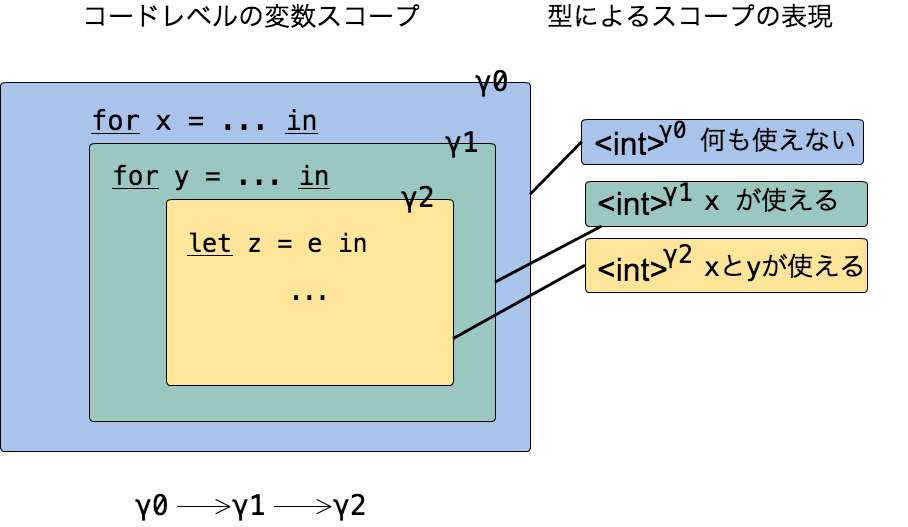
\includegraphics[clip,height=5.7cm]{./img/ec_for.png}
  % \end{center}
  % \begin{flushright}
  %   $\gamma_i ... \text{Refined Environment Classifier}$
  % \end{flushright}

  \newcommand\ml{\multicolumn}
  \center
  {\Large
    \begin{tabular}{l|l|l|l|l|l|}
      \cline{2-6}
      \alert{$\mathbf \gamma0$} & \ml{5}{|l|}{$\cfordo{x = e1}{e2}~~~~~~~~~~~~~~~$} \\ \cline{3-5}
                                & \alert{$\mathbf \gamma1$} & \ml{3}{|l|}{$\cfordo{y = e3}{e4}$} & \\ \cline{4-4}
                                &           & \alert{$\mathbf \gamma2$} & \ml{1}{|l|}{$\caryset{a}{(x,y)} cc$} & ~~ & \\ \cline{4-4}
                                &           & \ml{3}{|l|}{\ }    &               \\ \cline{3-5}
                                & \ml{5}{|l|}{~~~~~~~~~~~~~~~~~~ } \\ \cline{2-6}
    \end{tabular}
  }

  \begin{center}
    \begin{tabular}{c|c}
      スコープ & 使えるコード変数 \\ \hline
      \red{$\gamma0$} & なし \\ \hline
      \red{$\gamma1$} & $x$ \\ \hline
      \red{$\gamma2$} & $x, y$
    \end{tabular}\qquad
  \end{center}

  \red{$\gamma2$} $\ord$ \red{$\gamma1$} $\ord$ \red{$\gamma0$}
\end{frame}

% \begin{frame}
%   \frametitle{環境識別子(EC)を利用したスコープ表現\tiny{[Sudo+2014]}}
%   % 大なり記号はスコープの大きさを表しているのではなく,使える自由変数の集合の大きさを表している
%   型システムでコード変数のスコープを表現:

%   \center
%   \begin{align*}
%     & \Gamma = \gamma2 \ord \gamma1,~
%       x : \codeTs{\textbf{int}}{\gamma1},~
%       y : \codeTs{\textbf{int}}{\gamma2}
%   \end{align*}

%   \begin{tabular}{c|c}
%     $\gamma1$ & $\gamma2$ \\ \hline \hline
%     \uncover<1->{$\Gamma ~\vdash~ x : \codeTs{\textbf{int}}{\gamma1}~~ \alert{\text{OK}}$} & \uncover<1->{$\Gamma ~\vdash~ x : \codeTs{\textbf{int}}{\gamma2}~~ \alert{\text{OK}}$} \\ \hline

%     \uncover<1->{$\Gamma ~\vdash~ y : \codeTs{\textbf{int}}{\gamma1}~~ \alert{\text{NG}}$} & \uncover<1->{$\Gamma ~\vdash~ y : \codeTs{\textbf{int}}{\gamma2}~~ \alert{\text{OK}}$} \\ \hline

%     \uncover<1->{$\Gamma ~\vdash~ x\cPlus y : \codeTs{\textbf{int}}{\gamma1}~~  \alert{\text{NG}}$} & \uncover<1->{$\Gamma ~\vdash~ x\cPlus y : \codeTs{\textbf{int}}{\gamma2}~~  \alert{\text{OK}}$}
%   \end{tabular}

%   \bigskip

%   \begin{uncoverenv}<2->
%     コードレベルのラムダ抽象の型付け規則で固有変数条件を利用:

%     \[
%       \infer[(\gamma_2~\text{is eigen var})]
%       {\Gamma \vdash \cfun{x}{e} : \codeTs{t_1\to t_2}{\gamma_1} }
%       {\Gamma,~\gamma_2 \ord \gamma_1,~x:\codeTs{t_1}{\gamma_2} \vdash
%         e : \codeTs{t_2}{\gamma_2}}
%     \]
%   \end{uncoverenv}
% \end{frame}

\begin{frame}
  \frametitle{環境識別子(EC)を利用したスコープ表現}

  先行研究:
  \begin{itemize}
  \item 局所的なスコープをもつ破壊的変数をもつコード生成の体系に対する(型安全な)型システムの構築
    [Sudo,Kiselyov,Kameyama 2014]
  \item グローバルなスコープをもつ破壊的変数への拡張
    [Kiselyov,Kameyama,Sudo 2016]
  \item[◯] コントロールオペレータには非対応
  \end{itemize}

  \medskip
  \begin{uncoverenv}<2->
    \begin{exampleblock}{問題点:}
      shift0/reset0 などのコントロールオペレータは,スコープの包含関係を逆転させてしまう.
    \end{exampleblock}
  \end{uncoverenv}
\end{frame}


% \begin{frame}
%   \frametitle{本研究の解決策}
%   \flushleft
%   
\includegraphics[clip,height=3cm]{./img/ecgraph.png}
%   \begin{itemize}
%   \item<2-> $\gamma1$ のコード変数は $\gamma2$ では使ってはいけない
%   \item<2-> $\gamma2$ のコード変数は $\gamma1$ では使ってはいけない
%   \item<3->[$\Rightarrow$] \red{$\gamma1$ と $\gamma2$ の間に順序を付けない}
%   \end{itemize}

%   \begin{itemize}
%   \item<4-> $\gamma1, \gamma2$ のコード変数は $\gamma3$ で使ってよい
%   \item<5->[$\Rightarrow$] \red{Sudoらの体系に $\cup$ (ユニオン) を追加} % ジョイン
%   \end{itemize}
% \end{frame}

\begin{frame}[fragile]
  \frametitle{コード生成+shift0/reset0 の型システム\small{ (の一部)}}
  reset0:
  \[
    \infer{\Gamma \vdash \resetz{e} : \codeTs{t}{\gamma} ~ \lgray{;~ \sigma}}
    {\Gamma \vdash e : \codeTs{t}{\gamma} ~\lgray{;~ \codeTs{t}{\gamma}, \sigma}}
  \]

  shift0:
  \[
    \infer{\Gamma \vdash \shiftz{k}{e} : \codeTs{t1}{\red{\gamma1}} ~\lgray{;~ \codeTs{t0}{\gamma0},\sigma}}
    {\Gamma,~k:\contT{\codeTs{t1}{\gamma1}}{\codeTs{t0}{\gamma0}}
      \vdash e : \codeTs{t0}{\red{\gamma0}} ~\lgray{;~ \sigma}
      & \Gamma \models \gamma1 \ord \gamma0
    }
  \]

  throw:
  \[
    \infer
    {\Gamma,~k:\contT{\codeTs{t1}{\gamma1}}{\codeTs{t0}{\gamma0}}
      \vdash \throw{k}{v} : \codeTs{t0}{\gamma2} ~\lgray{;~ \sigma}}
    {\Gamma
      \vdash v : \codeTs{t1}{\red{\gamma1 \cup \gamma2}} ~\lgray{;~ \sigma}
      & \Gamma \models \gamma2 \ord \gamma0
    }
  \]
\end{frame}

\subsection{型付けの例}

\newcommand\boxterm{\framebox{
    \only<2>{\green{$\cint{3}$}}
    \only<3>{\red{$x~\cPlus~(\cint{3})$}}
    \phantom{A}
  }}

\begin{frame}
  \frametitle{型付けの例(1)}
  \begin{align*}
    e & = \Resetz ~~(\cfordo{x = e1}{e2} \\
      & \phantom{=}~~~ \Shiftz~k~\to~
        {\cLet~u=\green{\boxterm}~\cIn}~\Throw~k~u)
  \end{align*}

  \[
    \infer{\vdash e : \codeTs{t}{\gamma0};~\epsilon}
    {\infer[\blue{(\gamma1^*)}]{\vdash \cfor{x=...} :
        \codeTs{t}{\gamma0};~\codeTs{t}{\gamma0}}
      {\infer{\gamma1 \ord \gamma0,~x:\codeTs{t}{\gamma1}
          \vdash \Shiftz~k~\to~... :
          \codeTs{t}{\gamma1};~\codeTs{t}{\gamma0}}
        {\infer[(\gamma2^*)]{\Gamma a \vdash \cLet~u=...:\codeTs{t}{\gamma0};~\epsilon}
          {\infer{\Gamma b \vdash
              \Throw~k~u:\codeTs{t}{\gamma2};~\epsilon }
            {\infer{\Gamma b \vdash
                u:\codeTs{t}{\gamma1 \cup \gamma2};~ \sigma}
              {}
            }
            &\infer*{\Gamma a \vdash
              \green{\boxterm}:\codeTs{t}{\red{\gamma0}};~\epsilon}
            {}
          }
        }
      }
    }
  \]

  % $[(\gamma1^*)]$ は eigen variable (固有変数)

  {\footnotesize
    \begin{align*}
      \Gamma a &= \gamma1 \ord \gamma0,~x:\codeTs{t}{\red{\gamma1}},
                 ~k: \contT{\codeTs{t}{\gamma1}}{\codeTs{t}{\gamma0}} \\
      \Gamma b &= \Gamma a,~\gamma2 \ord \gamma0,~u:\codeTs{t}{\gamma2}
    \end{align*}
  }

\end{frame}

\begin{frame}
  \frametitle{型付けの例(2)}

  \newcommand\gammaa{\gamma1 \ord \gamma0,~x:\codeTs{t}{\gamma1}}
  \newcommand\gammab{\Gamma a,\gamma2 \ord \gamma1,~y:\codeTs{t}{\gamma2}}
  \newcommand\gammac{\Gamma b,\blue{k_2}:\contT{\codeTs{t}{\gamma2}}{\codeTs{t}{\gamma1}}}
  \newcommand\gammad{\Gamma c,\red{k_1}:\contT{\codeTs{t}{\gamma1}}{\codeTs{t}{\gamma0}}}
  \newcommand\gammae{\Gamma d,\gamma3 \ord \gamma0,\magenta{u}:\codeTs{t}{\gamma3}}

  \newcommand\boxterms{\framebox{
      \only<2>{\red{$x$}}
      \only<3>{\red{$y$}}
      \phantom{a}
    }}

  \vspace{-1zh} % odd

  \footnotesize
  \begin{align*}
    e'= & \red{\Resetz}~(\cfordo{x = e1}{e2}~\blue{\Resetz} ~(\cfordo{y = e3}{e4} \\
    % & \blue{\Shiftz}~\blue{k_2}\to~ \red{\Shiftz}~\red{k_1}\to~\magenta{\cLet~u=\green{\framebox{\phantom{x}}}~\cIn}
      & \blue{\Shiftz}~\blue{k_2}\to~ \red{\Shiftz}~\red{k_1}\to~\magenta{\cLet~u=\green{\boxterms}~\cIn}
          ~\red{\Throw~k_1}~(\blue{\Throw~k_2}~e5)))
  \end{align*}

  \vspace{-2zh} % odd

  \[
    \infer{\vdash e'=\red{\Resetz}\cdots : \codeTs{t}{\gamma0};~~~\epsilon}
    {\infer[(\gamma1^*)]
      {\vdash \cfor{x=...} : \codeTs{t}{\gamma0};~~~\codeTs{t}{\gamma0}}
      {\infer{\Gamma a=\gammaa\vdash \blue{\Resetz}\cdots : \codeTs{t}{\gamma1};~~~\codeTs{t}{\gamma0}}
        {\infer[(\gamma2^*)]
          {\Gamma a\vdash \cfor{y=...}: \codeTs{t}{\gamma1};~~~\codeTs{t}{\gamma1},\codeTs{t}{\gamma0}}
          {\infer{\Gamma b=\gammab\vdash \blue{\Shiftz~k_2}... :\codeTs{t}{\gamma2}
              ;~~~\codeTs{t}{\gamma1},\codeTs{t}{\gamma0}}
            {\infer{\Gamma c=\gammac\vdash \red{\Shiftz~k_1}... :\codeTs{t}{\gamma1}
                ;~~~\codeTs{t}{\gamma0}}
              {\infer[(\gamma3^*)]
                {\Gamma d=\gammad\vdash \magenta{\cLet~u=...} : \codeTs{t}{\gamma0};~\epsilon}
                {\infer
                  {\Gamma e=\gammae\vdash \red{\Throw~k_1}~... : \codeTs{t}{\gamma3};~\epsilon}
                  {\infer{\Gamma e\vdash \blue{\Throw~k_2}~e5 :
                      \codeTs{t}{\gamma1\cup\gamma3};~~\epsilon}
                    {\infer*{\Gamma e\vdash e5:
                        \codeTs{t}{\gamma2\cup\gamma1\cup\gamma3};~~~\epsilon}
                      {}
                    }
                  }
                  % &\infer*{\Gamma d\vdash \green{\framebox{\phantom{x}}}:\codeTs{t}{\gamma0};\epsilon}{}
                  &\infer*{\Gamma d\vdash \green{\boxterms}:\codeTs{t}{\gamma0};\epsilon}{}
                }
              }
            }
          }
        }
      }
    }
  \]

  {\footnotesize
    \begin{align*}
      \Gamma d &= \cdots,~ x:\codeTs{t}{\red{\gamma1}},~ y:\codeTs{t}{\red{\gamma2}},~ \gamma1 \ord \gamma0,~ \gamma2 \ord \gamma1,~ \cdots
    \end{align*}
  }

\end{frame}

%%% Local Variables:
%%% mode: latex
%%% TeX-master: "slide_oishi"
%%% End:
